\documentclass[
11pt, % Set the default font size, options include: 8pt, 9pt, 10pt, 11pt, 12pt, 14pt, 17pt, 20pt
%t, % Uncomment to vertically align all slide content to the top of the slide, rather than the default centered
%aspectratio=169, % Uncomment to set the aspect ratio to a 16:9 ratio which matches the aspect ratio of 1080p and 4K screens and projectors
]{beamer}

\graphicspath{{images/}{./}} % Specifies where to look for included images (trailing slash required)

\usepackage{watermark}
\usepackage{graphicx}  % Para incluir imágenes si deseas usar una imagen como marca de agua
\usepackage{array}
\usepackage[utf8]{inputenc}
\usepackage[spanish]{babel}
\usepackage{circuitikz} % Paquete para diagramas de circuitos eléctricos
\usepackage{tikz}
\usetikzlibrary{shapes.geometric, arrows.meta, positioning}
\usepackage{smartdiagram}
\usepackage{eso-pic}
\usepackage{lmodern}
\usepackage{xcolor}



% Agregar logo
\logo{
\includegraphics[width=1cm]{logo.jpeg}} % Cambia "logo.png" por la ruta de tu imagen

\usepackage{booktabs} % Allows the use of \toprule, \midrule and \bottomrule for better rules in tables

%----------------------------------------------------------------------------------------
%	SELECT LAYOUT THEME
%----------------------------------------------------------------------------------------

% Beamer comes with a number of default layout themes which change the colors and layouts of slides. Below is a list of all themes available, uncomment each in turn to see what they look like.

%\usetheme{default}
%\usetheme{AnnArbor}
%\usetheme{Antibes}
%\usetheme{Bergen}
%\usetheme{Berkeley}
%\usetheme{Berlin}
%\usetheme{Boadilla}
\usetheme{CambridgeUS}
%\usetheme{Copenhagen}
%\usetheme{Darmstadt}
%\usetheme{Dresden}
%\usetheme{Frankfurt}
%\usetheme{Goettingen}
%\usetheme{Hannover}
%\usetheme{Ilmenau}
%\usetheme{JuanLesPins}
%\usetheme{Luebeck}
%\usetheme{Madrid}
%\usetheme{Malmoe}
%\usetheme{Marburg}
%\usetheme{Montpellier}
%\usetheme{PaloAlto}
%\usetheme{Pittsburgh}
%\usetheme{Rochester}
%\usetheme{Singapore}
%\usetheme{Szeged}
%\usetheme{Warsaw}

%----------------------------------------------------------------------------------------
%	SELECT COLOR THEME
%----------------------------------------------------------------------------------------

% Beamer comes with a number of color themes that can be applied to any layout theme to change its colors. Uncomment each of these in turn to see how they change the colors of your selected layout theme.

%\usecolortheme{albatross}
%\usecolortheme{beaver}
%\usecolortheme{beetle}
%\usecolortheme{crane}
%\usecolortheme{dolphin}
%\usecolortheme{dove}
%\usecolortheme{fly}
%\usecolortheme{lily}
%\usecolortheme{monarca}
%\usecolortheme{seagull}
%\usecolortheme{seahorse}
%\usecolortheme{spruce}
%\usecolortheme{whale}
%\usecolortheme{wolverine}

%----------------------------------------------------------------------------------------
%	SELECT FONT THEME & FONTS
%----------------------------------------------------------------------------------------

% Beamer comes with several font themes to easily change the fonts used in various parts of the presentation. Review the comments beside each one to decide if you would like to use it. Note that additional options can be specified for several of these font themes, consult the beamer documentation for more information.

\usefonttheme{default} % Typeset using the default sans serif font
%\usefonttheme{serif} % Typeset using the default serif font (make sure a sans font isn't being set as the default font if you use this option!)
%\usefonttheme{structurebold} % Typeset important structure text (titles, headlines, footlines, sidebar, etc) in bold
%\usefonttheme{structureitalicserif} % Typeset important structure text (titles, headlines, footlines, sidebar, etc) in italic serif
%\usefonttheme{structuresmallcapsserif} % Typeset important structure text (titles, headlines, footlines, sidebar, etc) in small caps serif

%------------------------------------------------

%\usepackage{mathptmx} % Use the Times font for serif text
\usepackage{palatino} % Use the Palatino font for serif text

%\usepackage{helvet} % Use the Helvetica font for sans serif text
\usepackage[default]{opensans} % Use the Open Sans font for sans serif text
%\usepackage[default]{FiraSans} % Use the Fira Sans font for sans serif text
%\usepackage[default]{lato} % Use the Lato font for sans serif text

%----------------------------------------------------------------------------------------
%	SELECT INNER THEME
%----------------------------------------------------------------------------------------

% Inner themes change the styling of internal slide elements, for example: bullet points, blocks, bibliography entries, title pages, theorems, etc. Uncomment each theme in turn to see what changes it makes to your presentation.

%\useinnertheme{default}
\useinnertheme{circles}
%\useinnertheme{rectangles}
%\useinnertheme{rounded}
%\useinnertheme{inmargin}

%----------------------------------------------------------------------------------------
%	SELECT OUTER THEME
%----------------------------------------------------------------------------------------

% Outer themes change the overall layout of slides, such as: header and footer lines, sidebars and slide titles. Uncomment each theme in turn to see what changes it makes to your presentation.

%\useoutertheme{default}
%\useoutertheme{infolines}
%\useoutertheme{miniframes}
%\useoutertheme{smoothbars}
%\useoutertheme{sidebar}
%\useoutertheme{split}
%\useoutertheme{shadow}
%\useoutertheme{tree}
%\useoutertheme{smoothtree}

%\setbeamertemplate{footline} % Uncomment this line to remove the footer line in all slides
%\setbeamertemplate{footline}[page number] % Uncomment this line to replace the footer line in all slides with a simple slide count

%\setbeamertemplate{navigation symbols}{} % Uncomment this line to remove the navigation symbols from the bottom of all slides

%----------------------------------------------------------------------------------------
%	PRESENTATION INFORMATION
%----------------------------------------------------------------------------------------

\title[Metodología de Investigación]{Metodología para el estudio universitario} % The short title in the optional parameter appears at the bottom of every slide, the full title in the main parameter is only on the title page

%\subtitle{Optional Subtitle} % Presentation subtitle, remove this command if a subtitle isn't required

\author[Edison Achalma]{Edison Achalma} % Presenter name(s), the optional parameter can contain a shortened version to appear on the bottom of every slide, while the main parameter will appear on the title slide

\institute[CAU - UNSCH]{Corporación Académica Universitaria CAU - UNSCH \\ \smallskip \textit{achalmed.18@gmail.com}} % Your institution, the optional parameter can be used for the institution shorthand and will appear on the bottom of every slide after author names, while the required parameter is used on the title slide and can include your email address or additional information on separate lines

\date[\today]{Sesión 05 \\ \today} % Presentation date or conference/meeting name, the optional parameter can contain a shortened version to appear on the bottom of every slide, while the required parameter value is output to the title slide

%----------------------------------------------------------------------------------------


\begin{document}
% Página de título
\begin{frame}
	\titlepage
\end{frame}

% Diapositiva de contenido
% Configuración: Incluir índice automáticamente en cada sección

\AtBeginSection[]{
	\begin{frame}{Índice de la Sección}
		\tableofcontents[currentsection] % Índice automático de la sección actual
	\end{frame}
}

% Sección Introductoria
\section{Introducción}
\begin{frame}
	\frametitle{Introducción}
	\begin{itemize}
		\item En esta presentación exploraremos herramientas en línea para buscar recursos académicos.
		\item Útil para estudiantes de diversas áreas: ciencias, humanidades, ingeniería, etc.
		\item Incluye bases de datos, portales y ejemplos prácticos.
	\end{itemize}
\end{frame}

% Sección Google Scholar
\section{Google Scholar}
\begin{frame}
	\frametitle{Google Scholar}
	\begin{itemize}
		\item \textbf{Descripción:} Motor de búsqueda académico que indexa artículos, tesis, libros y más de diversas fuentes confiables.
		\item \textbf{URL:} \href{https://scholar.google.com}{scholar.google.com}
		\item \textbf{Ejemplo de búsqueda:} "Cambio climático en Ayacucho Perú"
	\end{itemize}
	\begin{figure}
		\centering
		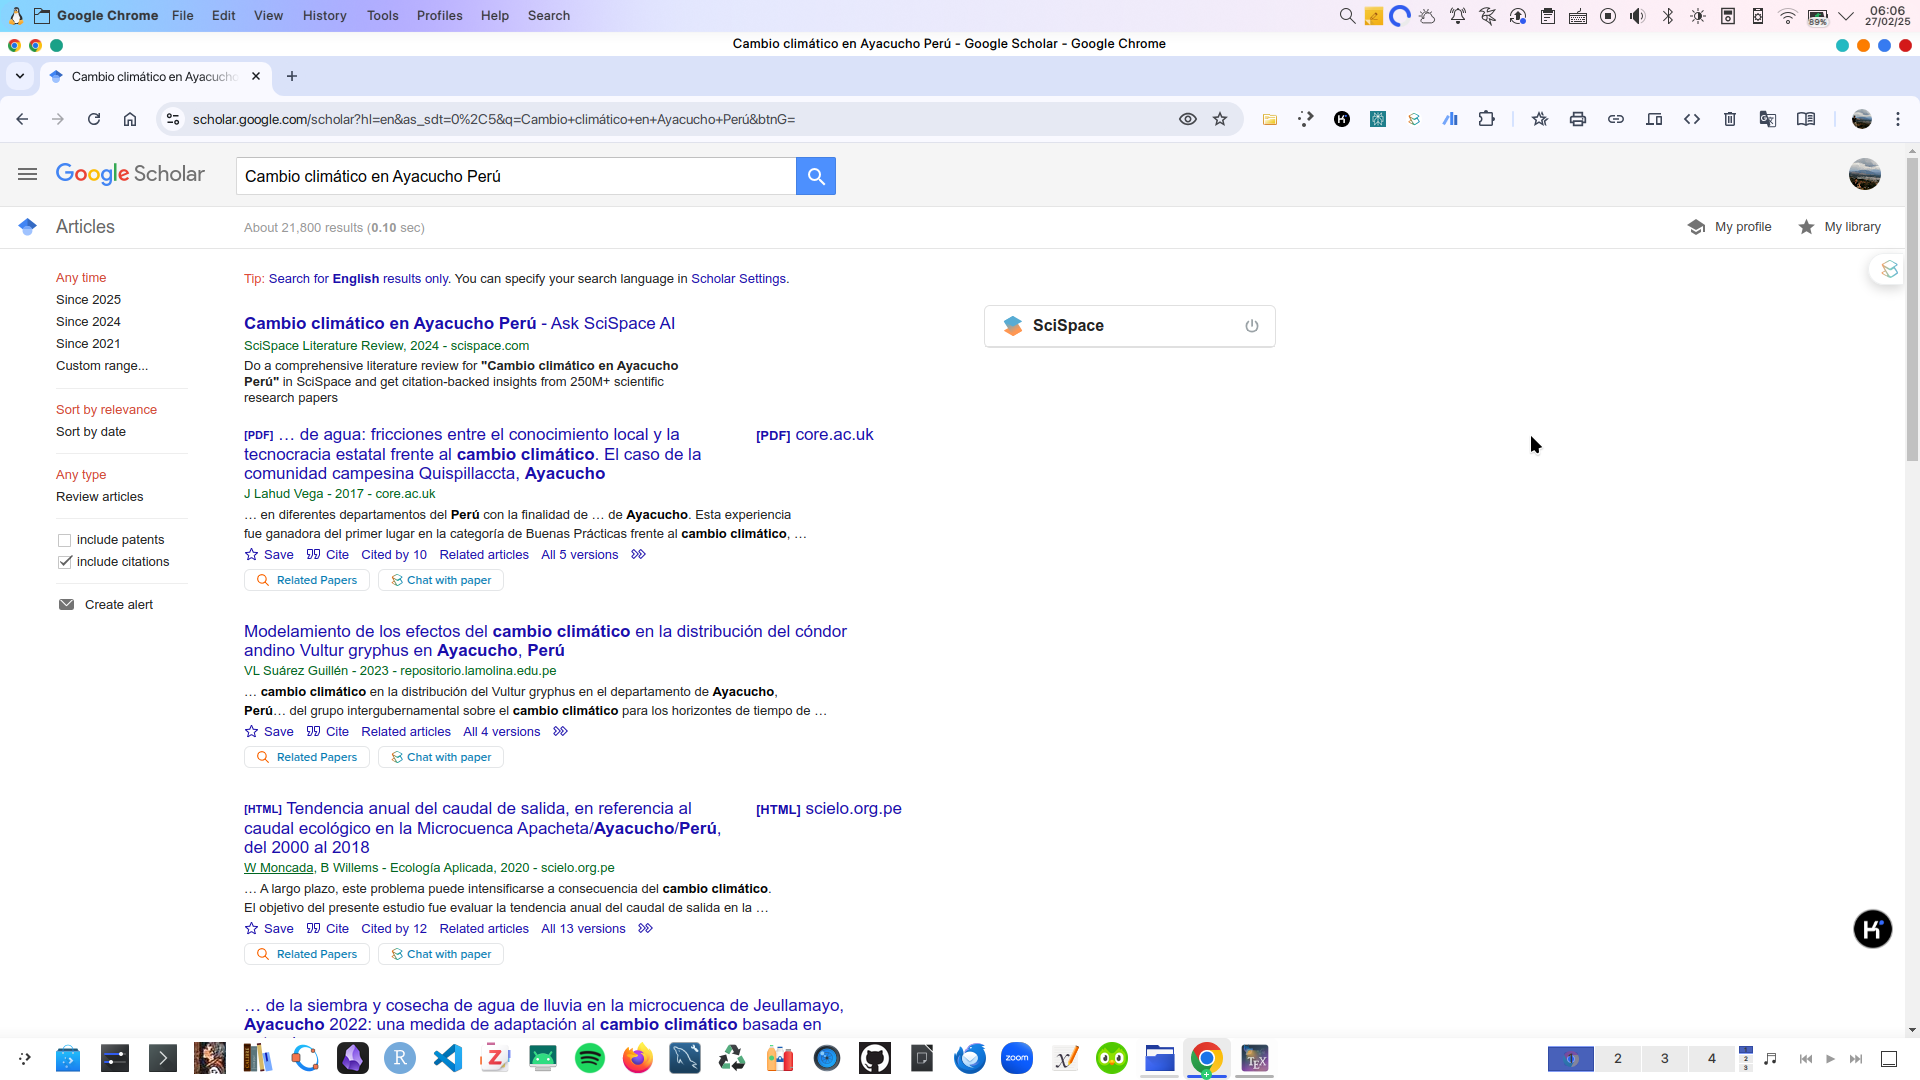
\includegraphics[width=0.9\linewidth]{images/google_scholar.png}
		\label{fig:screenshot010}
	\end{figure}
\end{frame}

% Sección PubMed
\section{PubMed}
\begin{frame}
	\frametitle{PubMed}
	\begin{itemize}
		\item \textbf{Descripción:} Base de datos especializada en ciencias de la salud, con millones de artículos médicos.
		\item \textbf{URL:} \href{https://pubmed.ncbi.nlm.nih.gov}{pubmed.ncbi.nlm.nih.gov}
		\item \textbf{Ejemplo de búsqueda:} "Diabetes mellitus tipo 2 Perú"
	\end{itemize}
	\begin{figure}
		\centering
		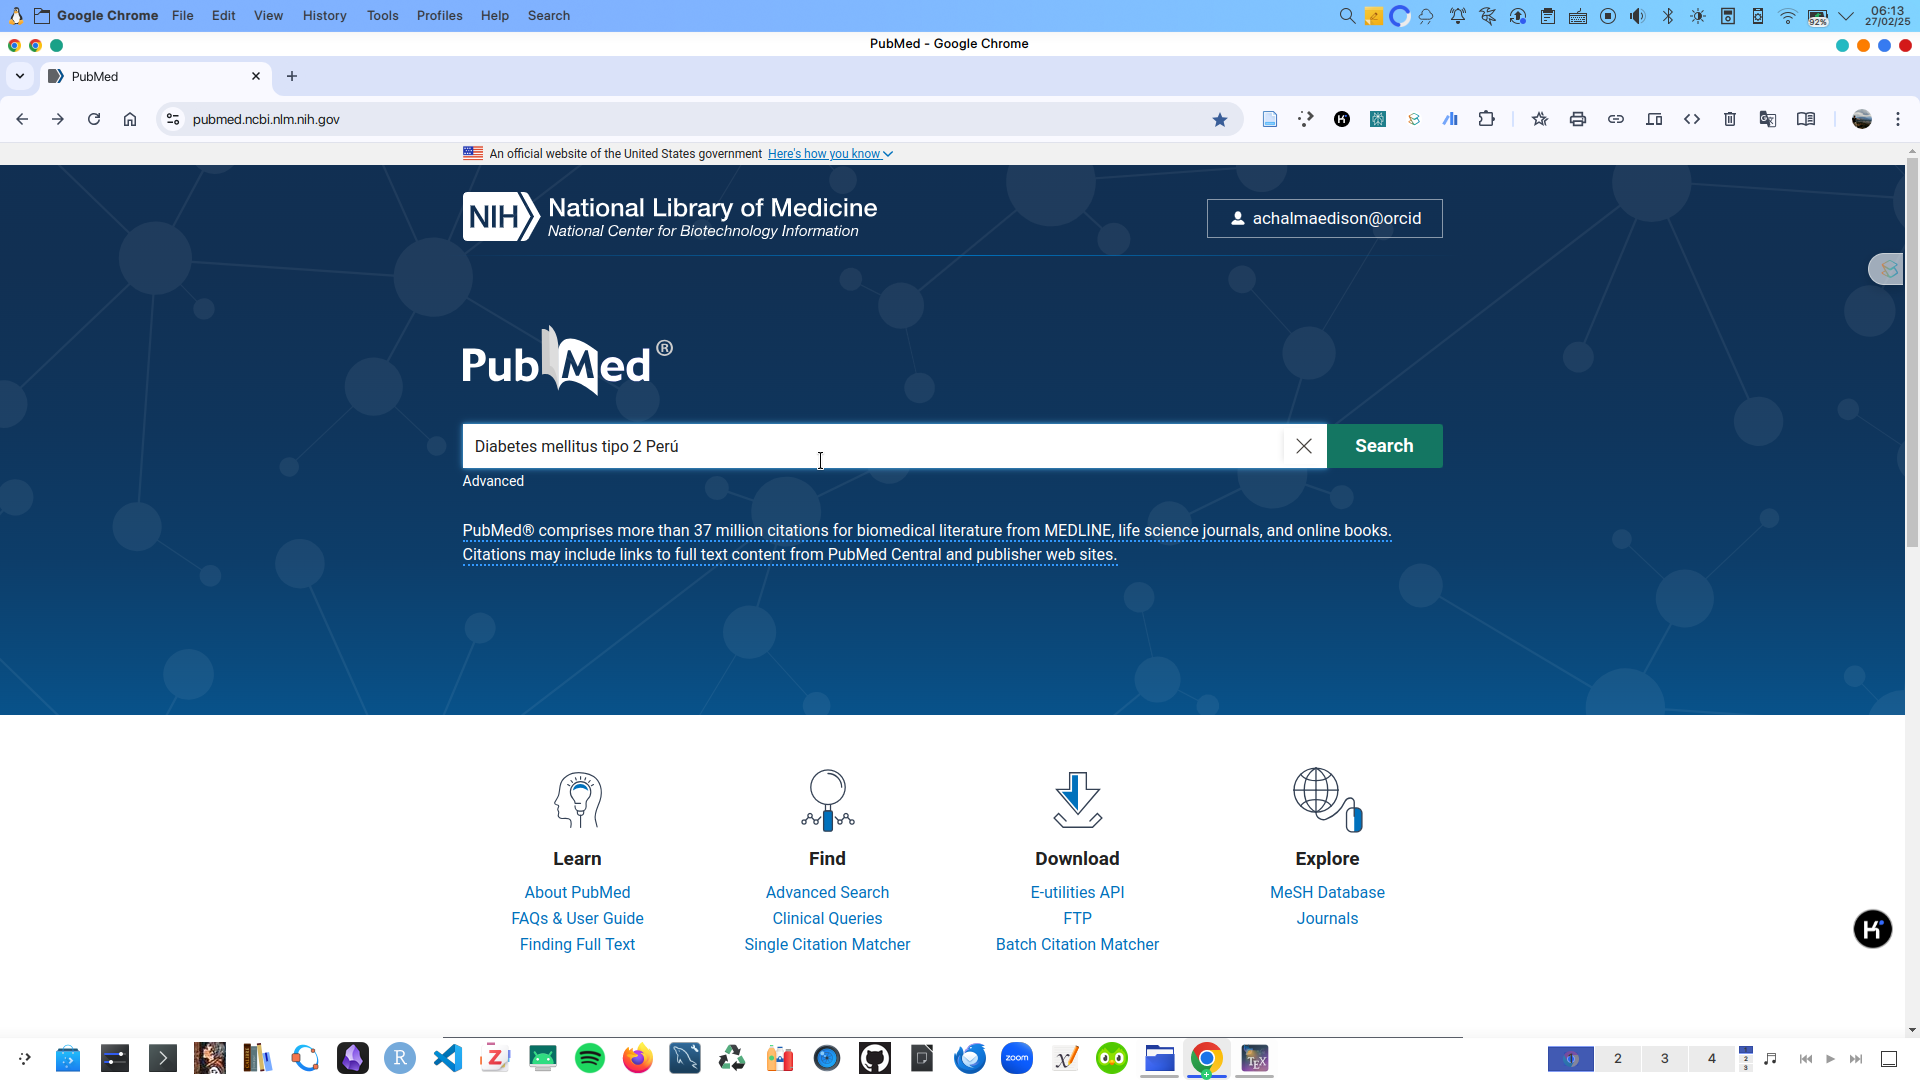
\includegraphics[width=0.9\linewidth]{images/pubmed.png}
		\label{fig:screenshot010}
	\end{figure}
\end{frame}

% Sección SciELO
\section{SciELO}
\begin{frame}
	\frametitle{SciELO}
	\begin{itemize}
		\item \textbf{Descripción:} Biblioteca electrónica de revistas científicas, con énfasis en América Latina y acceso abierto.
		\item \textbf{URL:} \href{https://scielo.org}{scielo.org}
		\item \textbf{Ejemplo de búsqueda:} "Agricultura sostenible en los Andes"
	\end{itemize}
		\begin{figure}
		\centering
		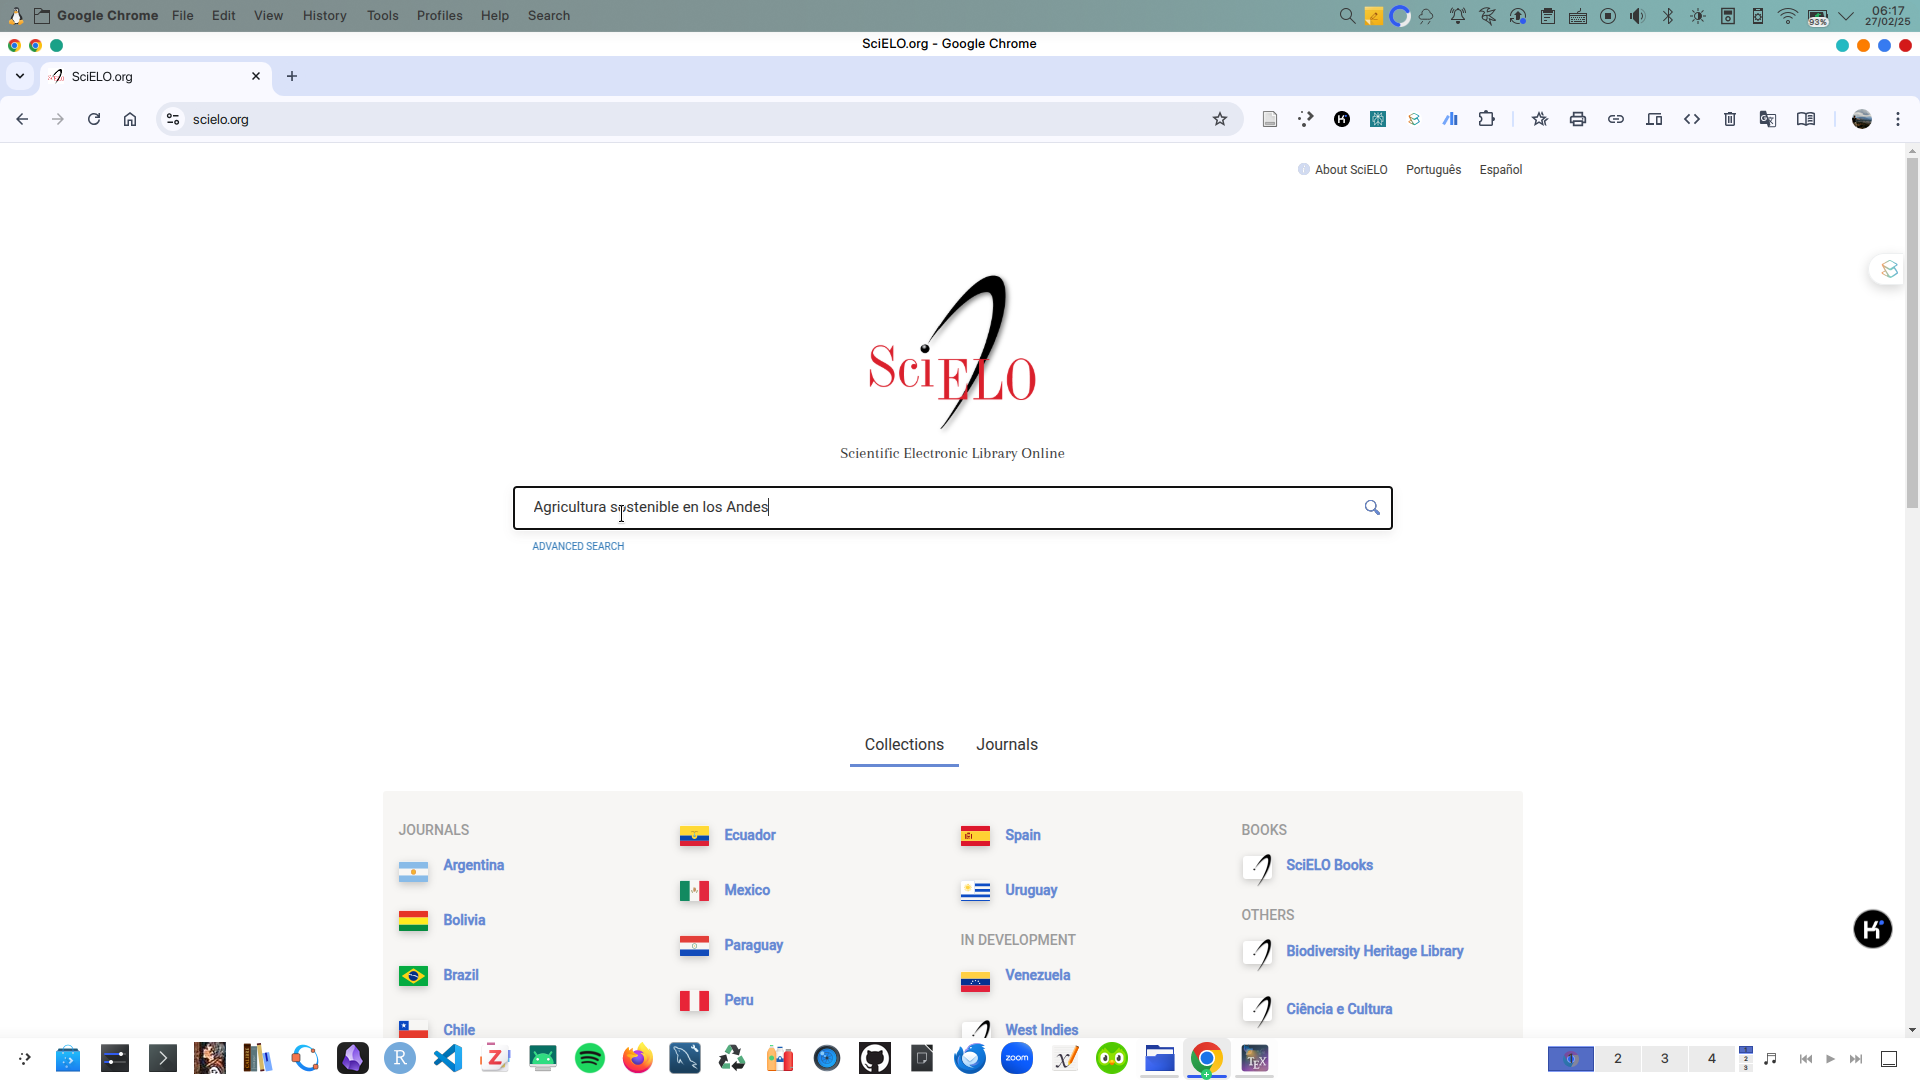
\includegraphics[width=0.9\linewidth]{images/scielo.png}
		\label{fig:screenshot010}
	\end{figure}
\end{frame}

% Sección Dialnet
\section{Dialnet}
\begin{frame}
	\frametitle{Dialnet}
	\begin{itemize}
		\item \textbf{Descripción:} Portal de difusión de literatura científica hispana, con artículos, libros y tesis.
		\item \textbf{URL:} \href{https://dialnet.unirioja.es}{dialnet.unirioja.es}
		\item \textbf{Ejemplo de búsqueda:} "Historia prehispánica de Ayacucho"
	\end{itemize}
		\begin{figure}
		\centering
		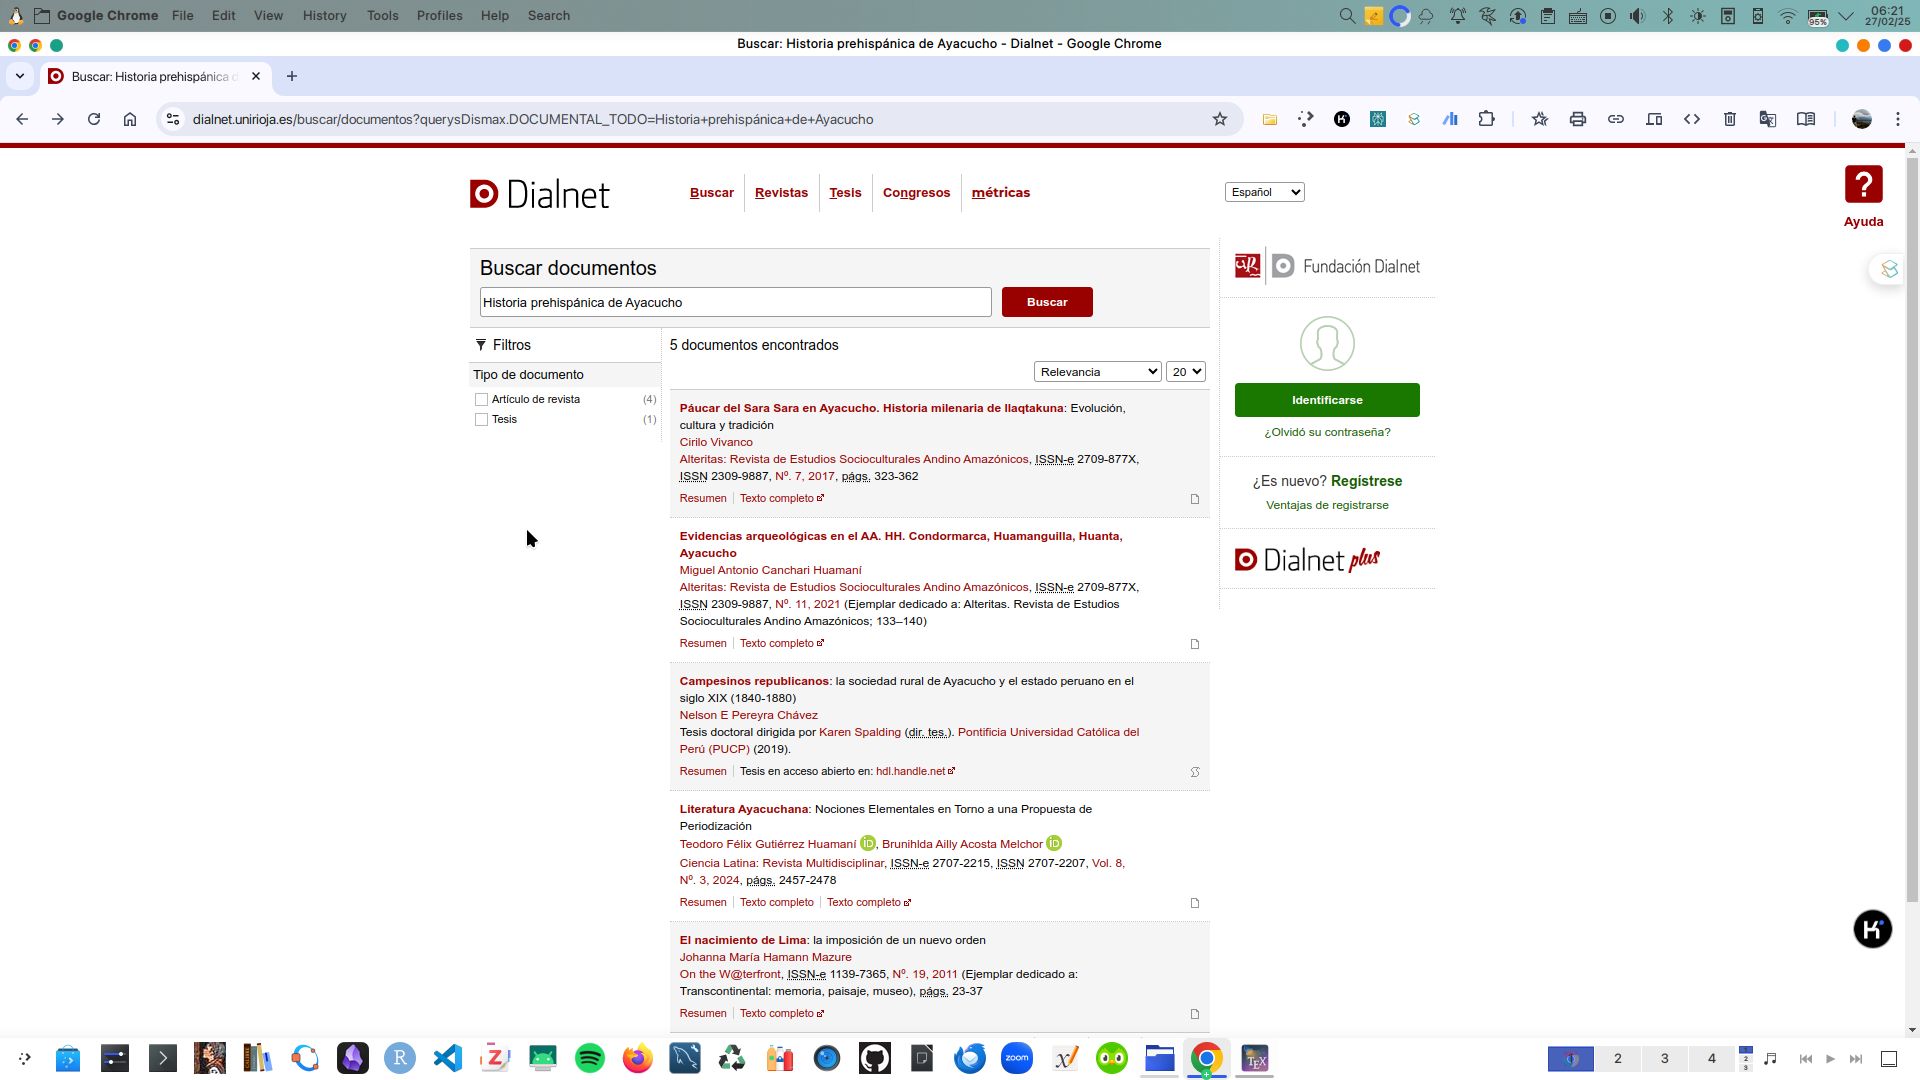
\includegraphics[width=0.9\linewidth]{images/dialnet.png}
		\label{fig:screenshot010}
	\end{figure}
\end{frame}

% Sección DOAJ
\section{DOAJ}
\begin{frame}
	\frametitle{Directory of Open Access Journals (DOAJ)}
	\begin{itemize}
		\item \textbf{Descripción:} Directorio de revistas científicas de acceso abierto, revisadas por pares.
		\item \textbf{URL:} \href{https://doaj.org}{doaj.org}
		\item \textbf{Ejemplo de búsqueda:} "Ingeniería de software"
	\end{itemize}
		\begin{figure}
		\centering
		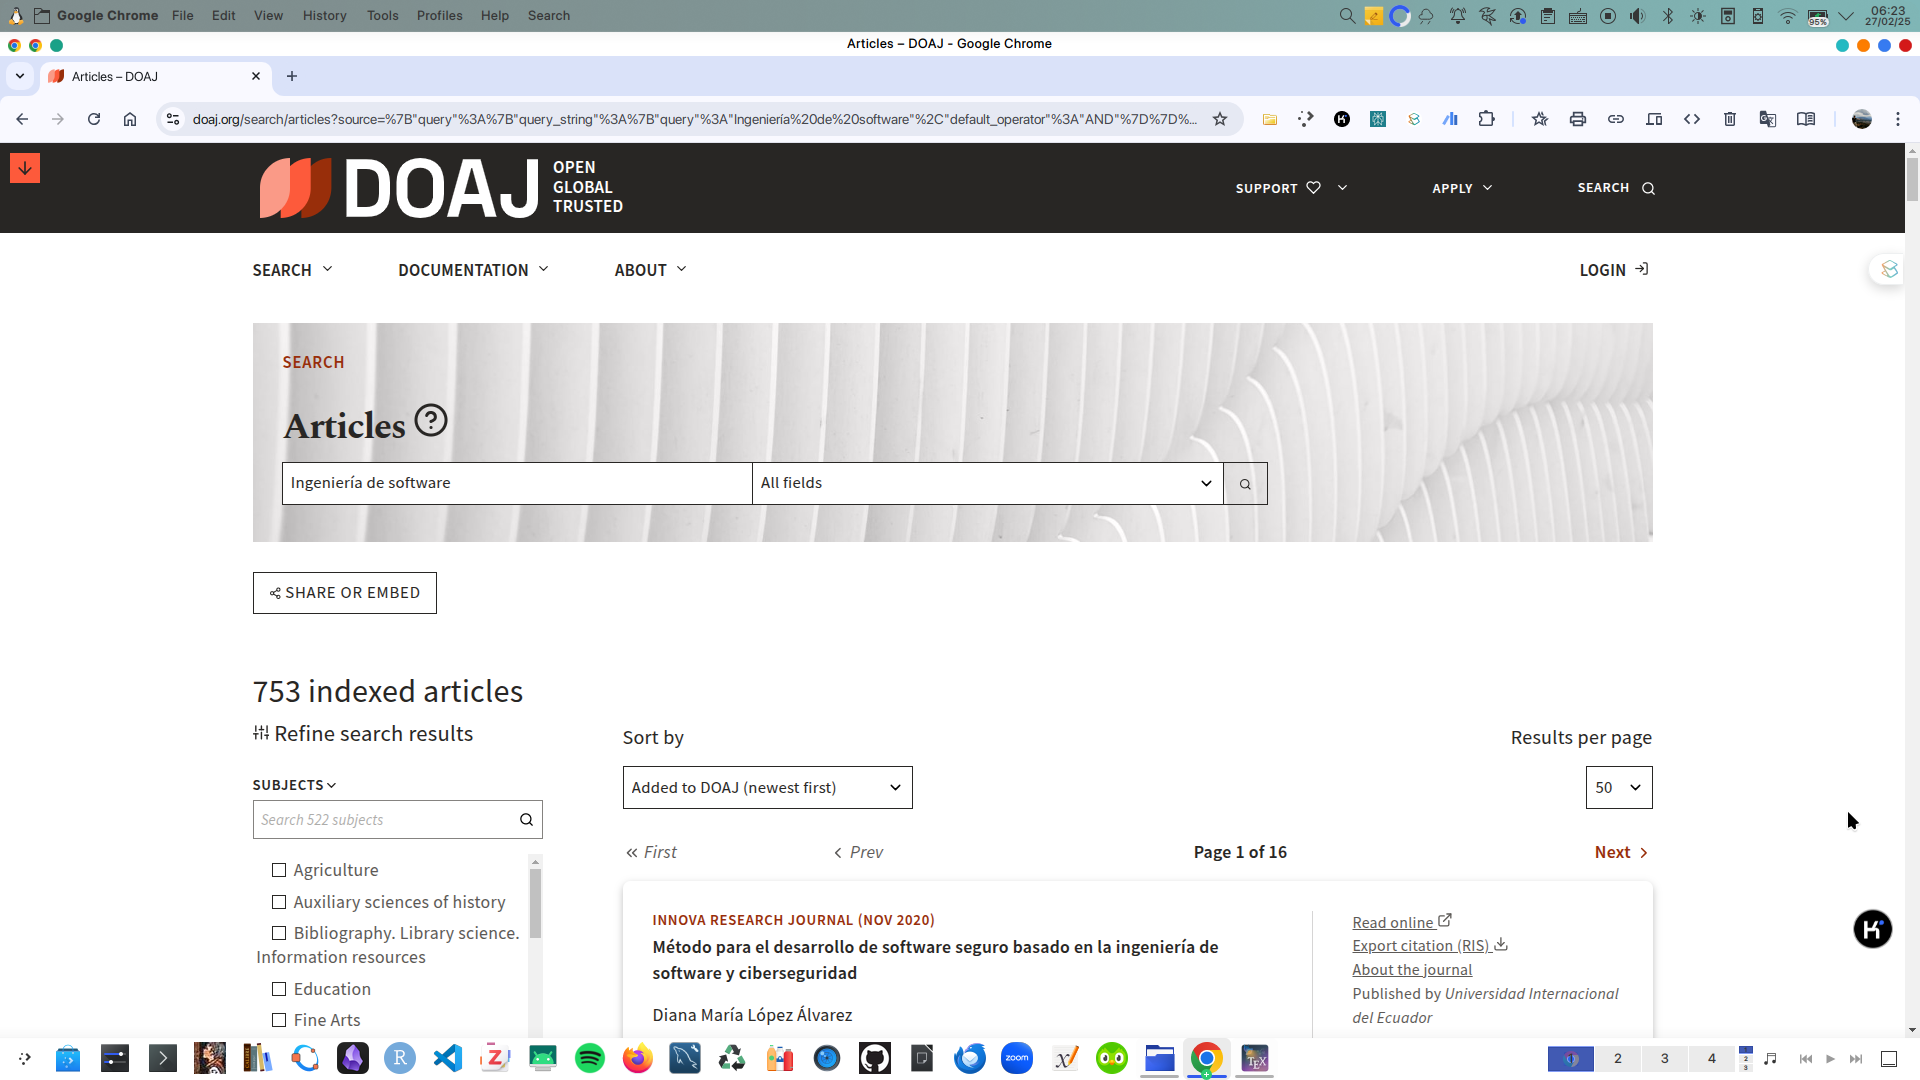
\includegraphics[width=0.9\linewidth]{images/doaj.png}
		\label{fig:screenshot010}
	\end{figure}
\end{frame}

% Sección SpringerLink
\section{SpringerLink}
\begin{frame}
	\frametitle{SpringerLink}
	\begin{itemize}
		\item \textbf{Descripción:} Plataforma con millones de documentos científicos: revistas, libros y actas.
		\item \textbf{URL:} \href{https://link.springer.com}{link.springer.com}
		\item \textbf{Ejemplo de búsqueda:} "Machine learning applications"
	\end{itemize}
			\begin{figure}
		\centering
		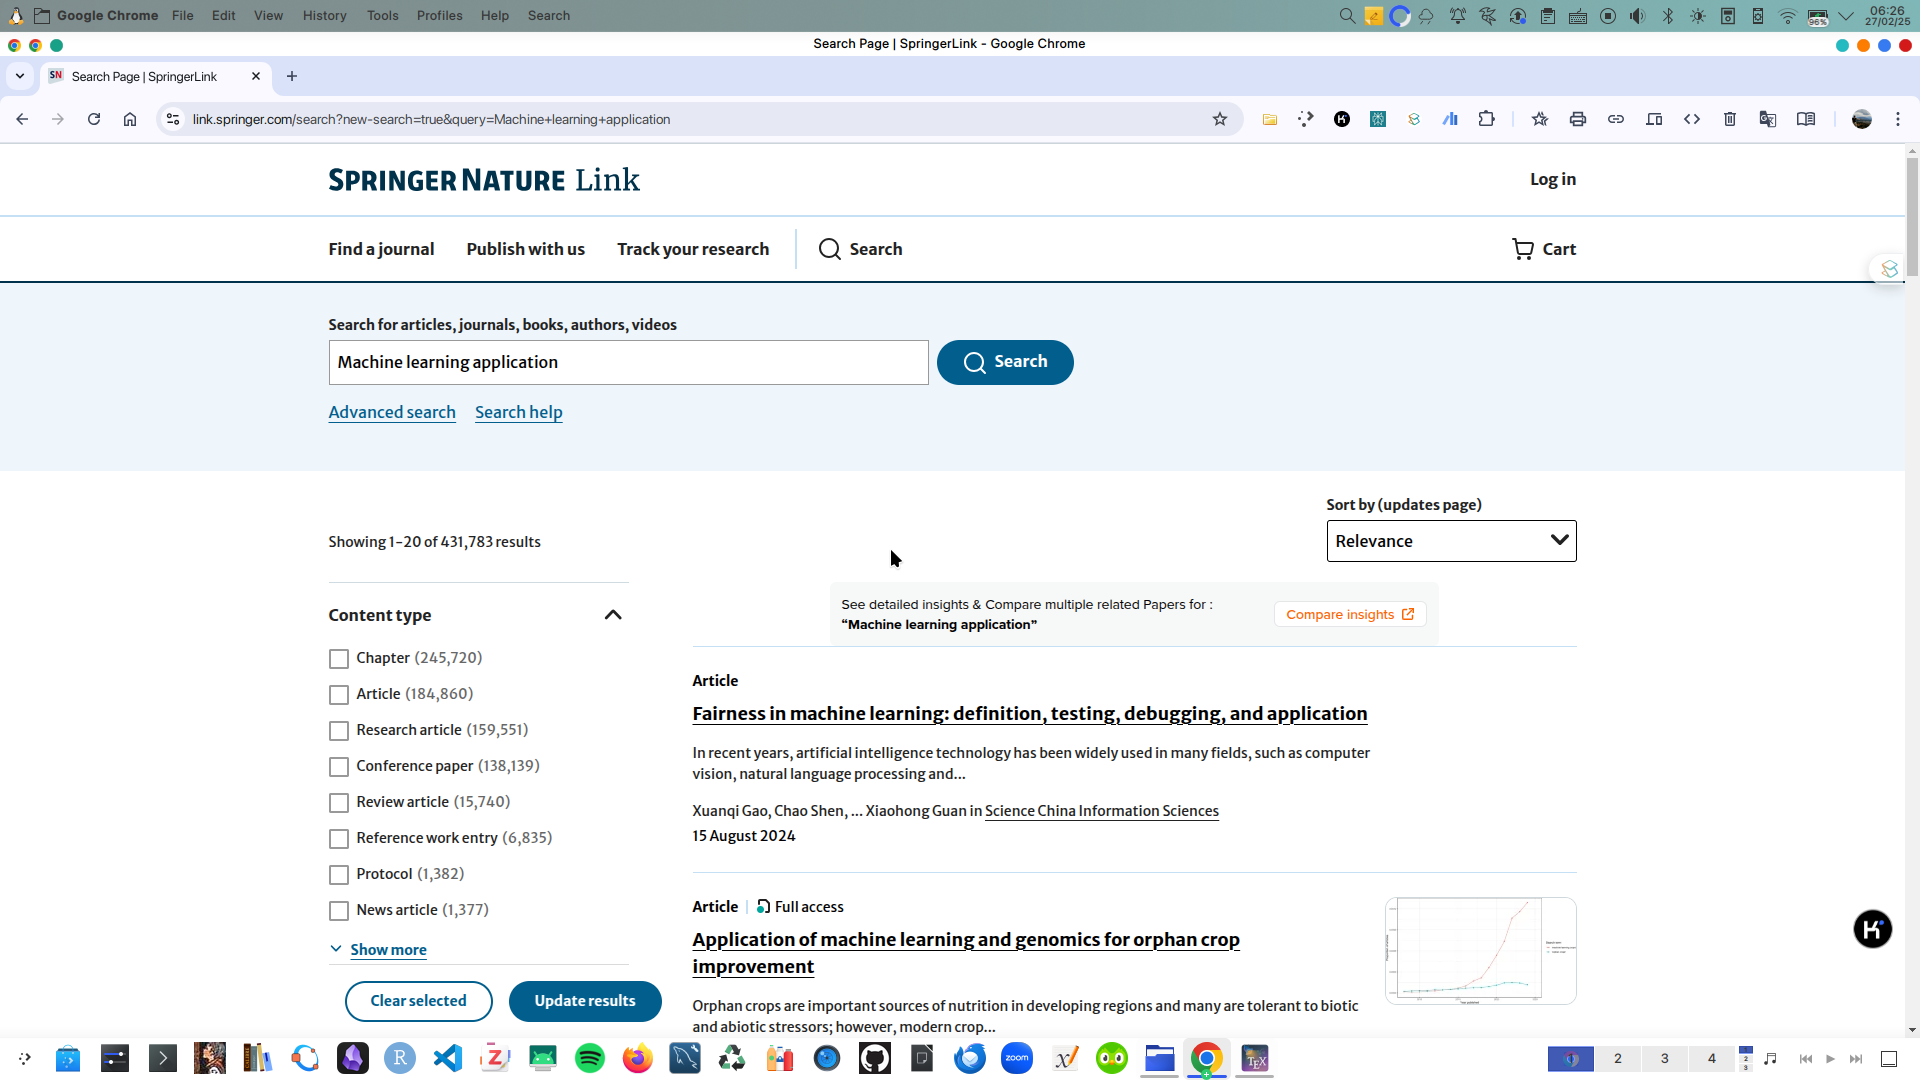
\includegraphics[width=0.9\linewidth]{images/springerlink.png}
		\label{fig:screenshot010}
	\end{figure}
\end{frame}

% Sección RENATI
\section{RENATI}
\begin{frame}
	\frametitle{RENATI}
	\begin{itemize}
		\item \textbf{Descripción:} Repositorio Nacional Digital de Tesis de Perú, gestionado por SUNEDU, con trabajos de grado y posgrado.
		\item \textbf{URL:} \href{https://renati.sunedu.gob.pe}{renati.sunedu.gob.pe}
		\item \textbf{Ejemplo de búsqueda:} "Educación rural en comunidades andinas"
	\end{itemize}
			\begin{figure}
		\centering
		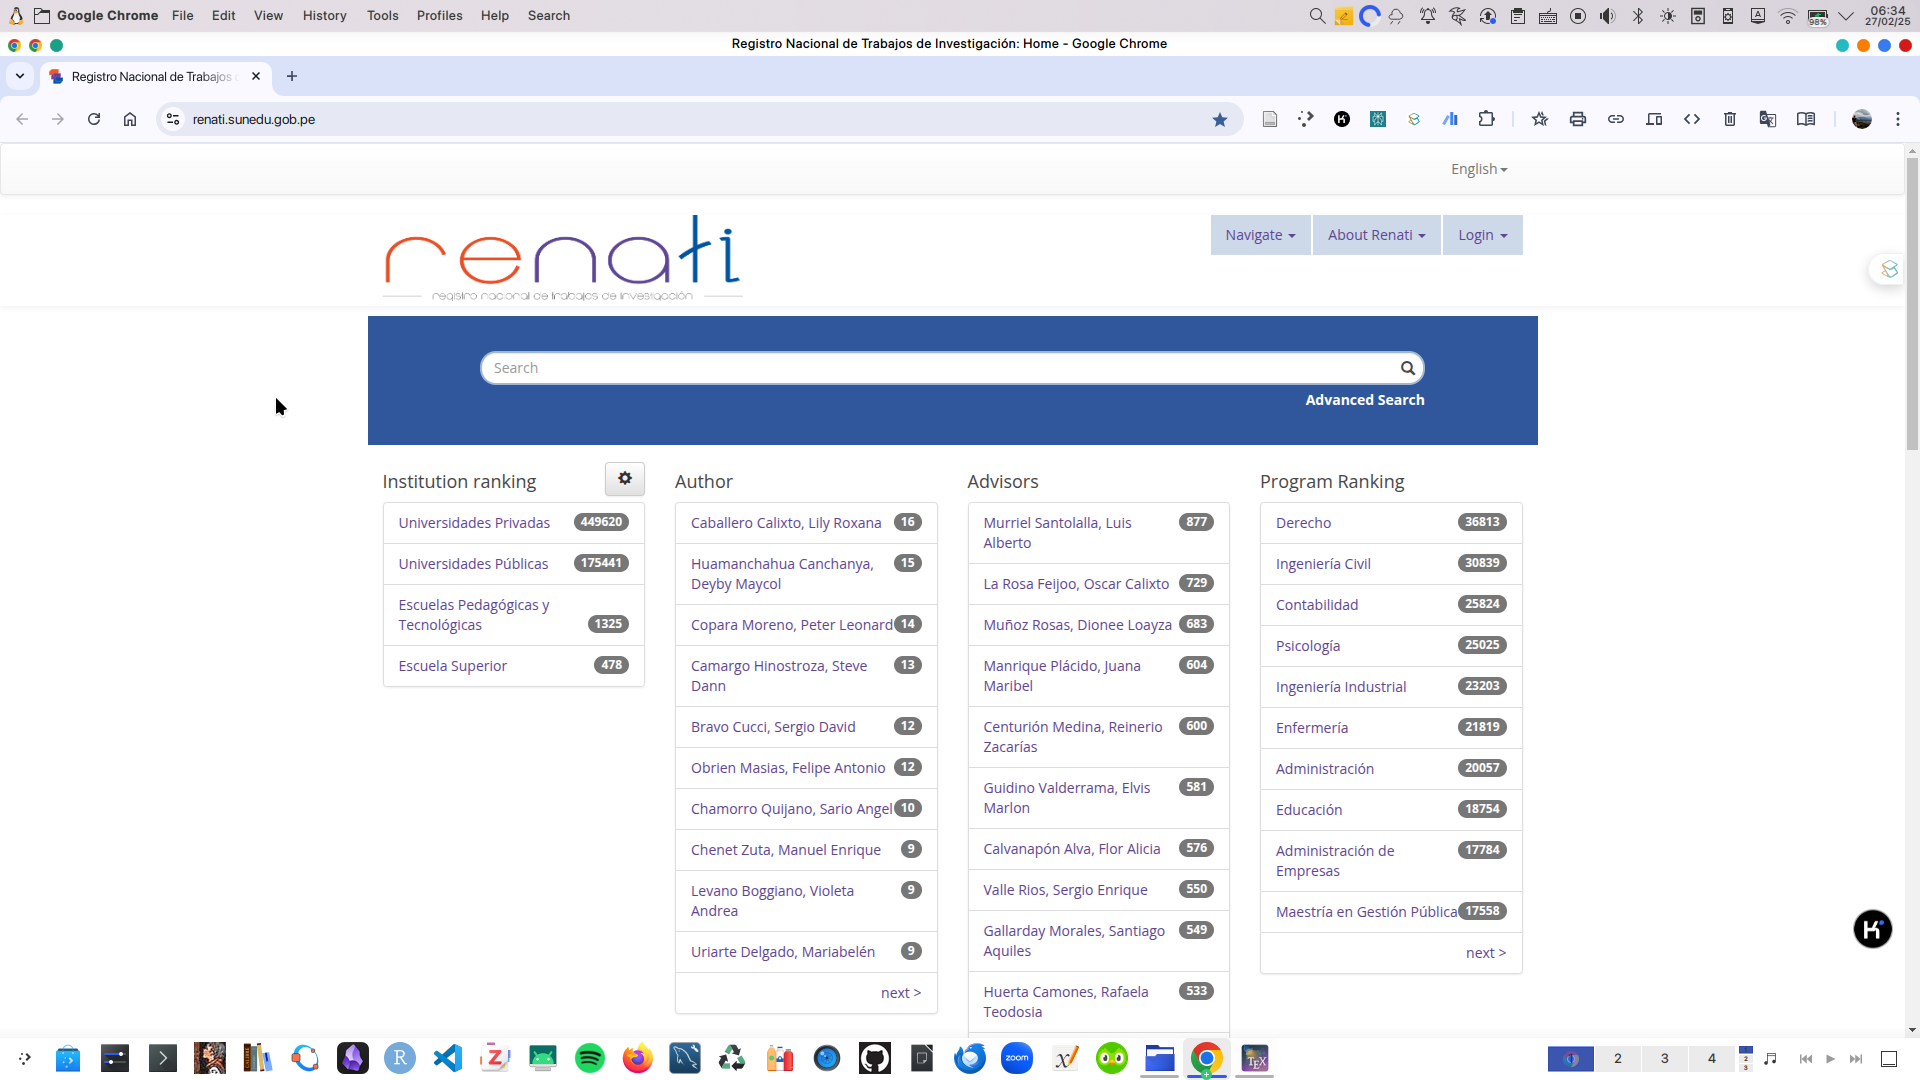
\includegraphics[width=0.9\linewidth]{images/renati.png}
		\label{fig:screenshot010}
	\end{figure}
\end{frame}

% Sección arXiv
\section{arXiv}
\begin{frame}
	\frametitle{arXiv}
	\begin{itemize}
		\item \textbf{Descripción:} Archivo de preprints de acceso abierto, enfocado en física, matemáticas, informática y más.
		\item \textbf{URL:} \href{https://arxiv.org}{arxiv.org}
		\item \textbf{Ejemplo de búsqueda:} "Machine learning en física teórica"
	\end{itemize}
				\begin{figure}
		\centering
		
\includegraphics[width=0.9\linewidth]{images/arxiv.png}
		\label{fig:screenshot010}
	\end{figure}
\end{frame}

% Sección Scopus
\section{Scopus}
\begin{frame}
	\frametitle{Scopus}
	\begin{itemize}
		\item \textbf{Descripción:} Base de datos de citas y resúmenes de Elsevier, con literatura revisada por pares de diversas disciplinas.
		\item \textbf{URL:} \href{https://www.scopus.com}{scopus.com}
		\item \textbf{Ejemplo de búsqueda:} "Innovación tecnológica en energía renovable"
	\end{itemize}
					\begin{figure}
		\centering
		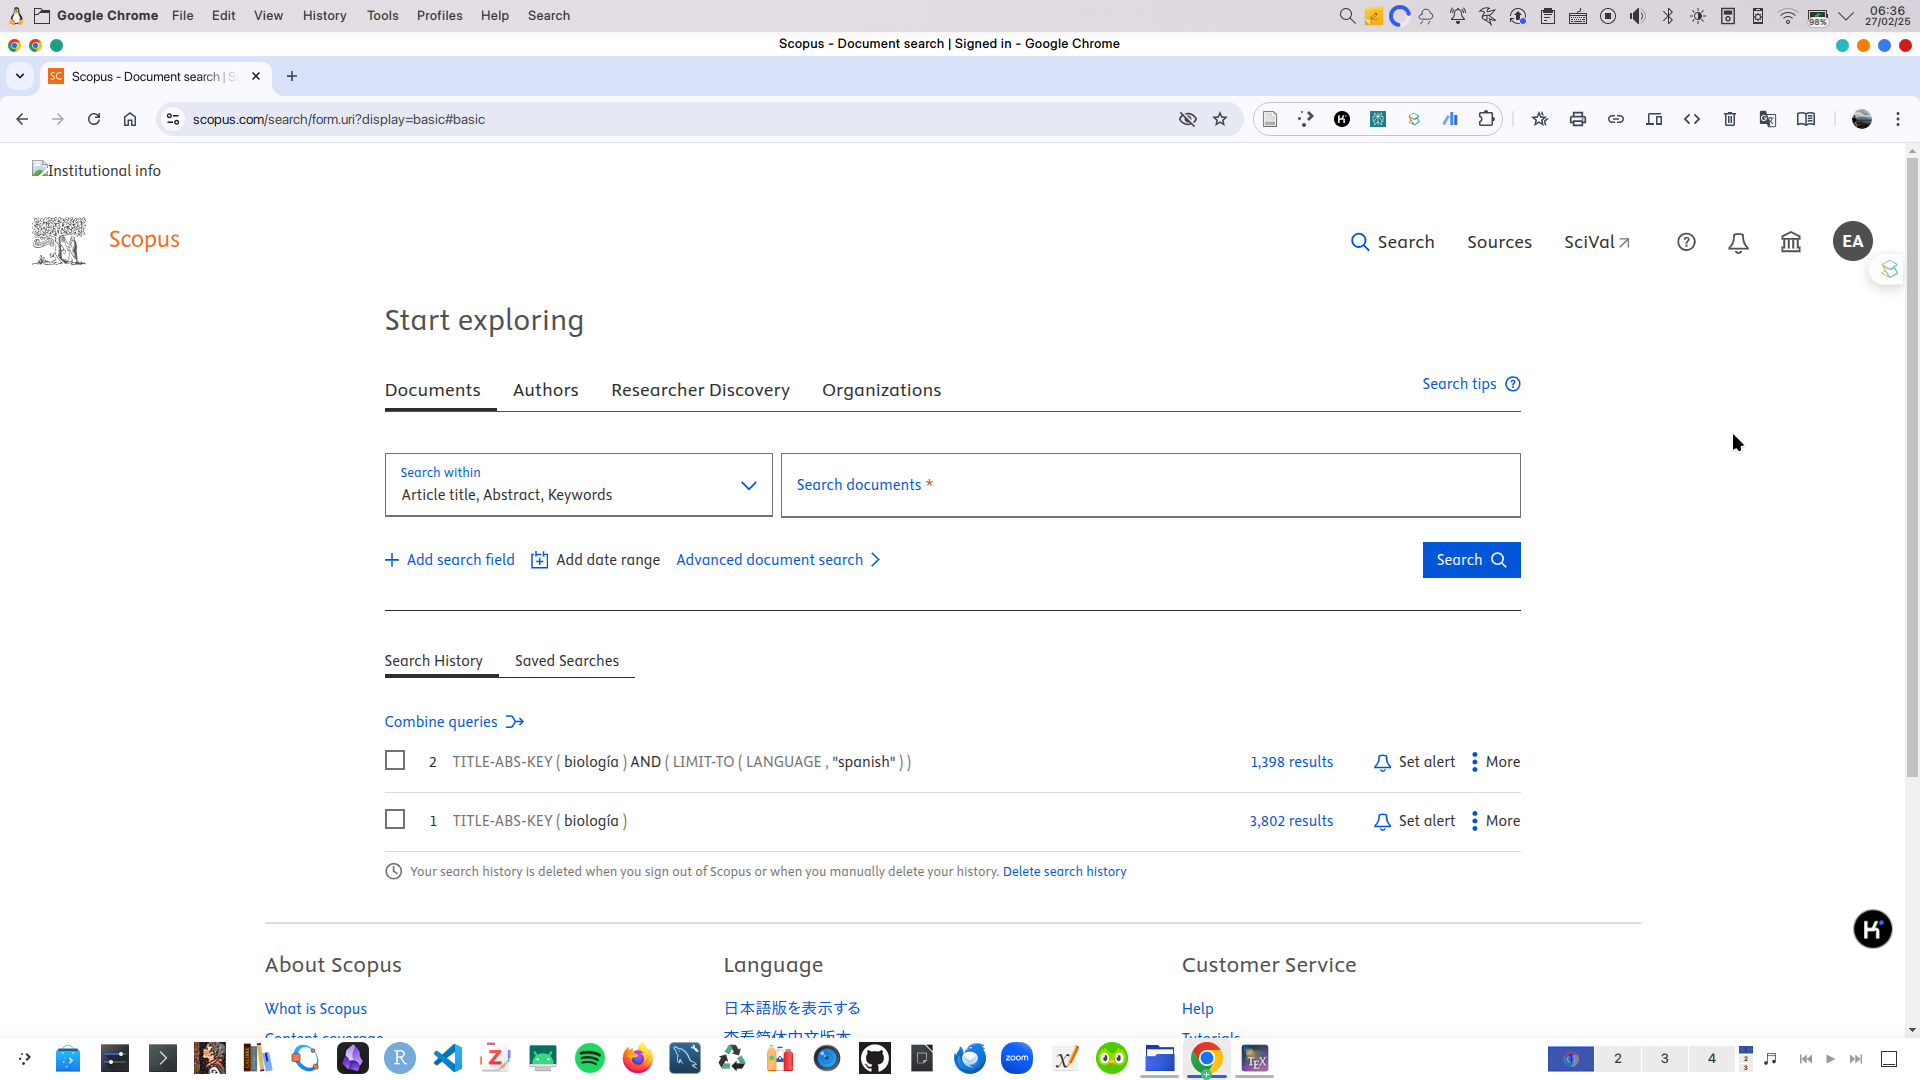
\includegraphics[width=0.9\linewidth]{images/scopus.png}
		\label{fig:screenshot010}
	\end{figure}
\end{frame}

% Sección Sci-Hub
\section{Sci-Hub}
\begin{frame}
	\frametitle{Sci-Hub}
	\begin{itemize}
		\item \textbf{Descripción:} Biblioteca sombra que ofrece acceso gratuito a artículos científicos, aunque su legalidad es debatida.
		\item \textbf{URL:} \href{https://sci-hub.se}{sci-hub.se}
	\end{itemize}
						\begin{figure}
		\centering
		
\includegraphics[width=0.9\linewidth]{images/scihub.png}
		\label{fig:screenshot010}
	\end{figure}
\end{frame}


% Sección 8
\section{Técnicas de parafraseo}

\begin{frame}
	\frametitle{¿Qué es el Parafraseo?}
	\begin{definition}
		Exposición o \textbf{explicación} que se realiza sobre un mensaje o \textbf{"ideas" del autor citado} con nuestras \textbf{propias palabras} para este resulte más sencillo de comprender. A esta acción se le conoce como \alert{parafrasear}.
	\end{definition}

	\begin{itemize}
		\item Es crucial en la escritura académica para evitar el plagio y para clarificar conceptos.
		\item \textcolor{red}{Te ha tocado un docente que te pone cero en un examen porque no has respondido exactamente igual a cómo dicto en clases o al libro que te hizo leer ...}
	\end{itemize}

	Cuando un texto ha sido parafraseado, debe incluir una cita adecuada.
\end{frame}

\begin{frame}
	\frametitle{Parafrasear}

	\begin{columns}[c] % The "c" option specifies centered vertical alignment while the "t" option is used for top vertical alignment
		\begin{column}{0.45\textwidth} % Left column width
			\begin{block}{¿Por qué?}
				\begin{itemize}
					\item Es un proceso lingüístico-cognitivo.
					\item Juega un papel central en la apropiación y conservación del conocimiento, según Fuchs (1985)
				\end{itemize}
			\end{block}
		\end{column}
		\begin{column}{0.5\textwidth} % Right column width
			\begin{block}{¿Para qué?}
				Para la construcción del conocimiento.

				\textbf{El estudiante de CAU-UNSCH debe estar en la capacidad de explicar lo que comprendió con sus propias palabras.}
			\end{block}
		\end{column}
	\end{columns}
	\begin{alertblock}{Nota}
		\textcolor{red}{¡Leer y comprender, OK!}
	\end{alertblock}

\end{frame}

\begin{frame}
	\frametitle{Tipos de parafraseo}
	\begin{block}{Mecánico}
		Es la \textbf{sustitución simple} de expresiones o palabras del texto original por sus sinónimos.

		\textcolor{red}{Se realiza} cambios sintácticos \textcolor{red}{mínimos}.
	\end{block}

	\begin{block}{Constructivo}
		Es la reelaboración del texto con palabras o características muy distintas. Pero conservando el mismo significado del texto original.

		\textcolor{blue}{Se realizan} cambios \textcolor{blue}{sintácticos} \textcolor{blue}{sustanciales}.
	\end{block}
\end{frame}

\begin{frame}
	\begin{figure}[H]
		\centering
		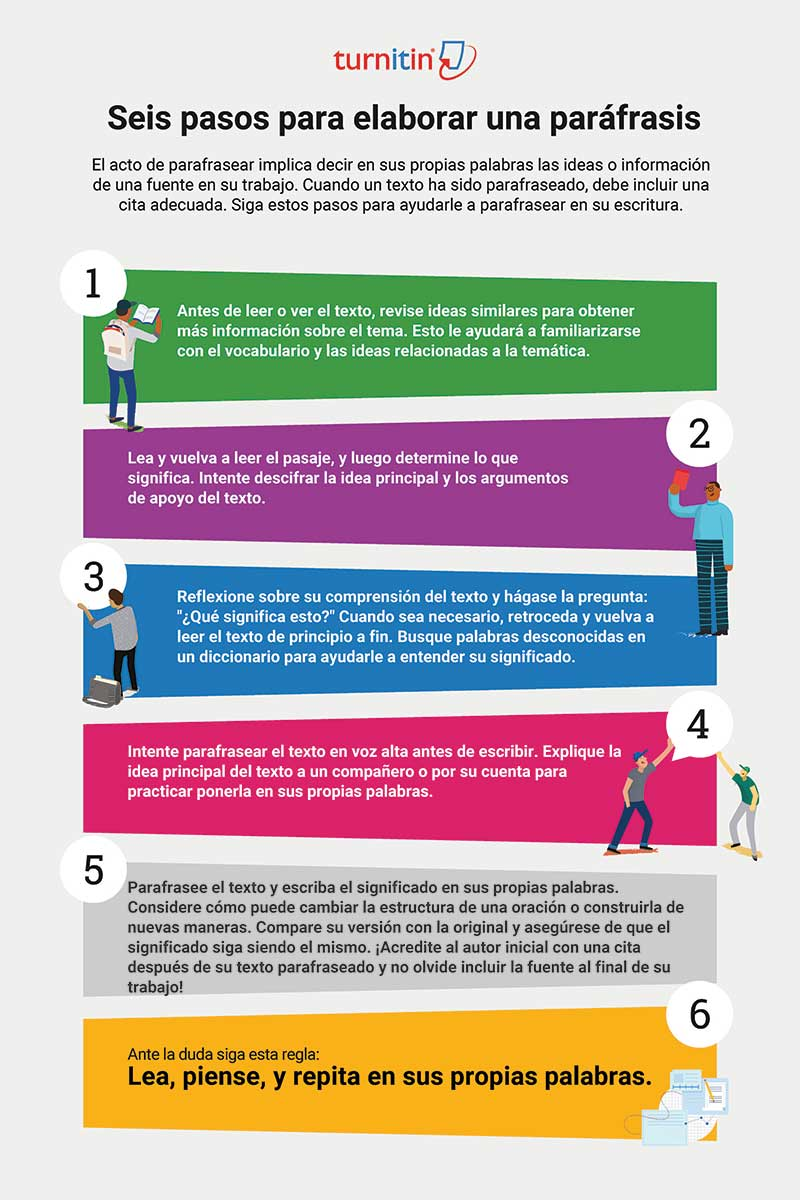
\includegraphics[width=0.5\linewidth]{images/seis-pasos-para-elaborar-una-parafrasis-opt}
	\end{figure}
\end{frame}

\begin{frame}
	\textbf{Identifique las ideas clave y palabras clave:}
	\begin{block}{} % Block without title
		En el análisis de \textbf{Robbins} sobre el comportamiento organizacional, se identifican rasgos del \textbf{liderazgo situacional}, donde el \textbf{líder} adapta su estilo según las circunstancias y el nivel de madurez de sus \textbf{colaboradores}. Este enfoque fomenta que los equipos enfrenten los \textbf{desafíos} con estrategias flexibles, promoviendo una reflexión constante sobre las \textbf{metas organizacionales} y los \textbf{recursos disponibles}. Además, estos líderes no solo responden a las \textbf{necesidades inmediatas}, sino que buscan potenciar el \textbf{desarrollo profesional} de sus seguidores, creando entornos que favorezcan el \textbf{crecimiento sostenible}. (Robbins y Judge, 2013, p.15).
	\end{block}
\end{frame}

\begin{frame}
	\begin{block}{} % Block without title
		\textcolor{teal}{En el análisis de \textbf{Robbins} se identifican rasgos del \textbf{liderazgo situacional}}, donde el \textbf{líder} adapta su estilo según las circunstancias y el nivel de madurez de sus \textbf{colaboradores}. \textcolor{olive}{Este enfoque fomenta que los equipos enfrenten los \textbf{desafíos} con estrategias flexibles, promoviendo una reflexión constante sobre las \textbf{metas organizacionales} y los \textbf{recursos disponibles}}. \textcolor{cyan}{Además, estos líderes no solo responden a las \textbf{necesidades inmediatas}, sino que buscan potenciar el \textbf{desarrollo profesional} de sus seguidores}, \textcolor{magenta}{creando entornos que favorezcan el \textbf{crecimiento sostenible}}. (Robbins y Judge, 2013, p.15).
	\end{block}
\end{frame}

\begin{frame}
	\begin{block}{} % Block without title
		\textbf{Robbins} destaca en su estudio componentes del \textbf{liderazgo situacional}, en el que el \textbf{líder} ajusta su enfoque según el contexto y las capacidades de sus \textbf{colaboradores}. Esto permite que los equipos aborden los \textbf{desafíos} con soluciones adaptativas, incentivando la evaluación de las \textbf{metas organizacionales} y el uso eficiente de los \textbf{recursos disponibles}. Adicionalmente, estos líderes atienden las \textbf{necesidades inmediatas} mientras impulsan el \textbf{desarrollo profesional}, generando condiciones óptimas para un \textbf{crecimiento sostenible}. (Robbins y Judge, 2013).
	\end{block}
\end{frame}

\begin{frame}
	\textbf{Identifique las ideas clave y palabras clave:}
	\begin{block}{} % Block without title
		El mercado se regula por la mano invisible, un mecanismo que permite que las acciones individuales de los agentes económicos, motivadas por el interés propio, generen beneficios colectivos en forma de equilibrio de oferta y demanda. Este principio sostiene que la libertad de los individuos para perseguir sus objetivos económicos fomenta la competencia, lo que a su vez impulsa la innovación y la eficiencia en la producción. Así, el bienestar social mejora sin necesidad de intervención directa del estado. (Smith, 1776, p.34).
	\end{block}
\end{frame}

\begin{frame}
	\begin{block}{} % Block without title
		\textcolor{purple}{El mercado se regula por la \textbf{mano invisible}}, un mecanismo que permite que las acciones individuales de los \textbf{agentes económicos}, motivadas por el interés propio, generen beneficios colectivos en forma de \textbf{equilibrio de oferta y demanda}. \textcolor{brown}{Este principio sostiene que la libertad de los individuos para perseguir sus \textbf{objetivos económicos} fomenta la \textbf{competencia}}, lo que impulsa la \textcolor{blue}{\textbf{innovación} y la \textbf{eficiencia en la producción}}. \textcolor{red}{Así, el \textbf{bienestar social} mejora sin necesidad de intervención directa del estado}. (Smith, 1776, p.34).
	\end{block}
\end{frame}

\begin{frame}
	\begin{block}{} % Block without title
		\textbf{Smith} argumenta que la \textbf{mano invisible} guía el mercado, haciendo que las decisiones de los \textbf{agentes económicos}, basadas en su interés personal, conduzcan a un \textbf{equilibrio de oferta y demanda}. Esta idea destaca que al permitir a los individuos buscar sus \textbf{objetivos económicos}, se promueve la \textbf{competencia}, lo que estimula la \textbf{innovación} y la \textbf{eficiencia en la producción}. De este modo, el \textbf{bienestar social} aumenta sin que el estado tenga que intervenir directamente. (Smith, 1776).
	\end{block}
\end{frame}


\begin{frame}
	\textbf{Identifique las ideas clave y palabras clave:}
	\begin{block}{} % Block without title
		La evolución ocurre mediante la selección natural, un proceso donde los organismos con características más ventajosas tienen mayor probabilidad de sobrevivir y reproducirse, transmitiendo sus rasgos a la descendencia. Este mecanismo impulsa la adaptación de las especies al entorno, permitiendo su supervivencia frente a cambios ambientales. Con el tiempo, estas variaciones generan diversidad biológica observable en la naturaleza. (Darwin, 1859, p.56).
	\end{block}
\end{frame}

\begin{frame}
	\begin{block}{} % Block without title
		\textcolor{purple}{La evolución ocurre mediante la \textbf{selección natural}}, un proceso donde los \textbf{organismos} con características más ventajosas tienen mayor probabilidad de sobrevivir y reproducirse, transmitiendo sus \textbf{rasgos} a la descendencia. \textcolor{brown}{Este mecanismo impulsa la \textbf{adaptación} de las especies al \textbf{entorno}}, permitiendo su supervivencia frente a cambios ambientales. \textcolor{blue}{Con el tiempo, estas variaciones generan \textbf{diversidad biológica} observable en la naturaleza}. (Darwin, 1859, p.56).
	\end{block}
\end{frame}

\begin{frame}
	\begin{block}{} % Block without title
		\textbf{Darwin} explica que la \textbf{selección natural} dirige la evolución, favoreciendo a los \textbf{organismos} con \textbf{rasgos} ventajosos que les permiten sobrevivir y reproducirse. Este proceso facilita la \textbf{adaptación} de las especies a su \textbf{entorno}, asegurando su permanencia ante cambios ambientais. A lo largo del tiempo, tales cambios producen la \textbf{diversidad biológica} que se observa en el mundo natural. (Darwin, 1859).
	\end{block}
\end{frame}


\begin{frame}
	\textbf{Identifique las ideas clave y palabras clave:}
	\begin{block}{} % Block without title
		El derecho se compone de reglas primarias y secundarias, donde las primeras imponen deberes y las segundas establecen procedimientos para crear, modificar o interpretar esas normas. Este sistema asegura la coherencia del ordenamiento jurídico, permitiendo que las autoridades apliquen sanciones cuando se incumplen las obligaciones legales. Así, la estabilidad social se mantiene mediante la estructura normativa. (Hart, 1961, p.89).
	\end{block}
\end{frame}

\begin{frame}
	\begin{block}{} % Block without title
		\textcolor{purple}{El derecho se compone de \textbf{reglas primarias} y \textbf{secundarias}}, donde las primeras imponen deberes y las segundas establecen \textbf{procedimientos} para crear, modificar o interpretar normas. \textcolor{brown}{Este sistema asegura la \textbf{coherencia} del \textbf{ordenamiento jurídico}}, permitiendo que las \textcolor{blue}{\textbf{autoridades} apliquen \textbf{sanciones} cuando se incumplen las obligaciones}. \textcolor{red}{Así, la \textbf{estabilidad social} se mantiene mediante la estructura normativa}. (Hart, 1961, p.89).
	\end{block}
\end{frame}

\begin{frame}
	\begin{block}{} % Block without title
		\textbf{Hart} afirma que el derecho está formado por \textbf{reglas primarias} y \textbf{secundarias}, siendo las primeras las que imponen obligaciones y las segundas las que definen \textbf{procedimientos} para gestionar esas normas. Esta estructura garantiza la \textbf{coherencia} del \textbf{ordenamiento jurídico}, facilitando que las \textbf{autoridades} impongan \textbf{sanciones} ante incumplimientos. De esta forma, la \textbf{estabilidad social} se preserva gracias al sistema normativo. (Hart, 1961).
	\end{block}
\end{frame}



\begin{frame}
	\textbf{Identifique las ideas clave y palabras clave:}
	\begin{block}{} % Block without title
		El modelo en espiral para el desarrollo de software, es un enfoque que combina iteraciones con la evaluación constante de riesgos para garantizar la calidad del producto final. Este método permite a los equipos ajustar los requisitos según retroalimentación, promoviendo la flexibilidad y la entrega incremental de soluciones funcionales. Así, se optimiza el proceso de desarrollo tecnológico. (Boehm, 1988, p.102).
	\end{block}
\end{frame}

\begin{frame}
	\begin{block}{} % Block without title
		\textcolor{purple}{El \textbf{modelo en espiral} para el desarrollo de \textbf{software}}, es un enfoque que combina iteraciones con la evaluación constante de \textbf{riesgos} para garantizar la calidad del producto. \textcolor{brown}{Este método permite a los \textbf{equipos} ajustar los \textbf{requisitos} según retroalimentación}, promoviendo la \textcolor{blue}{\textbf{flexibilidad} y la entrega incremental de \textbf{soluciones funcionales}}. \textcolor{red}{Así, se optimiza el \textbf{proceso de desarrollo} tecnológico}. (Boehm, 1988, p.102).
	\end{block}
\end{frame}

\begin{frame}
	\begin{block}{} % Block without title
		\textbf{Boehm} introduce el \textbf{modelo en espiral} en el desarrollo de \textbf{software}, integrando iteraciones y la revisión continua de \textbf{riesgos} para asegurar un producto de calidad. Esta estrategia ayuda a los \textbf{equipos} a modificar los \textbf{requisitos} con base en comentarios, fomentando la \textbf{flexibilidad} y la entrega progresiva de \textbf{soluciones funcionales}. De este modo, el \textbf{proceso de desarrollo} tecnológico se mejora significativamente. (Boehm, 1988).
	\end{block}
\end{frame}


\begin{frame}
	\textbf{Identifique las ideas clave y palabras clave:}
	\begin{block}{} % Block without title

		Encontramos en esta última categoría descrita por Aktouf elementos del liderazgo transformacional, al emerger situaciones donde el líder impulsa a sus seguidores a pensar sobre los problemas en formas nuevas y creativas, y los estimula a cuestionarse tanto sobre sus creencias y valores individuales como sobre las del líder, más cuando las soluciones planteadas son inapropiadas para resolver los problemas presentes. Adicionalmente este tipo de líderes no solamente reconocen y satisfacen las necesidades actuales de sus seguidores, sino que facilitan la expansión y elevación de sus abanicos de necesidades para que éstos puedan desarrollar todo su potencial. Los líderes transformacionales proveen oportunidades para el desarrollo de culturas organizacionales que sean soporte del crecimiento individual y colectivo. (Mendoza y Ortiz, 2006, p.8).
	\end{block}
\end{frame}

\begin{frame}
	\begin{block}{} % Block without title
		\textcolor{purple}{Encontramos en esta última categoría descrita por \textbf{Aktouf} elementos del \textbf{liderazgo transformacional}}, al emerger situaciones donde el \textbf{líder} impulsa a sus seguidores a pensar sobre los \textbf{problemas} en formas nuevas y creativas, \textcolor{brown}{y los estimula a cuestionarse tanto sobre sus \textbf{creencias y valores individuales} como sobre las del líder, más cuando las \textbf{soluciones planteadas} son inapropiadas para resolver los problemas presentes}. \textcolor{blue}{Adicionalmente este tipo de líderes no solamente reconocen y satisfacen las \textbf{necesidades} actuales de sus \textbf{seguidores}, sino que facilitan la expansión y elevación de sus abanicos de necesidades para que éstos puedan desarrollar todo su potencial}. \textcolor{red}{Los \textbf{líderes transformacionales} proveen oportunidades para el desarrollo de \textbf{culturas organizacionales} que sean soporte del \textbf{crecimiento individual y colectivo}}. (Mendoza y Ortiz, 2006, p.8).
	\end{block}
\end{frame}

\begin{frame}
	\begin{block}{} % Block without title
		\textbf{Aktouf} en la categoría final presenta elementos del \textbf{liderazgo transformacional}, en las ocasiones que el \textbf{líder} sugiere a sus seguidores a analizar los problemas creativamente, y los alienta a evaluar \textbf{sus creencias y valores individuales} y las suyas, si las \textbf{soluciones planteadas} no resuelven dichos problemas. Estos líderes, además de reconocer y satisfacer las \textbf{necesidades} que sus \textbf{seguidores} tienen en el presente, se toman el trabajo de ampliar y desarrollar la gama de sus necesidades con la finalidad que ellos logren \textbf{desarrollar todo su potencial}. \textbf{Líderes transformacionales} brindan opciones que impulsan las culturas organizacionales para que estimulen el \textbf{crecimiento individual y colectivo} (Mendoza y Ortiz, 2006).
	\end{block}
\end{frame}


\begin{frame}
	\begin{block}{} % Block without title
		La cultura de la organización se compone de valores, creencias, supuestos, percepciones, normas y patrones de comportamiento comunes a todos los que trabajan en ella; es a la organización lo que la personalidad es al individuo: un tema oculto pero unificador que proporciona sentido, dirección y movilización (Anzola, 2003, p. 51).
	\end{block}
\end{frame}

\begin{frame}
	\begin{block}{} % Block without title
		La \textbf{cultura de la organización} se compone de \textbf{valores}, \textbf{creencias}, \textbf{supuestos}, \textbf{percepciones}, normas y patrones de \textbf{comportamiento comunes} a todos los que trabajan en ella; es a la \textbf{organización} lo que la \textbf{personalidad es al individuo}: un tema oculto pero unificador que proporciona \textbf{sentido}, \textbf{dirección} y \textbf{movilización} (Anzola, 2003, p. 51).
	\end{block}
\end{frame}

\begin{frame}
	\frametitle{¡Qué es lo que no se parafrasea!}
	\begin{itemize}
		\item Definiciones
		\item Leyes científicas
		\item Listas
		\item Objetivos, hipótesis, conclusiones y similares
		\item Contenido de tablas, infografías y similares
		\item Textos que presentan relaciones o causalidades
		\item Todo párrafo que esté lleno de Palabras Clave
	\end{itemize}
\end{frame}

\begin{frame}
	\frametitle{Técnica 1: Cambiar la función gramatical}
	\begin{block}{Original}
		El profesor de medicina John Swenson plantea que los cambios globales influyen en la propagación de las enfermedades.
	\end{block}
	\begin{block}{Parafraseado}
		De acuerdo con John Swenson, un profesor de medicina, los cambios al rededor del globo causan que las enfermedades se propaguen. (James, 2004)
	\end{block}
\end{frame}

\begin{frame}
	\frametitle{Técnica 2: Uso de sinónimos}
	\begin{block}{Original}
		\only<1>{Un portavoz del gobierno norteamericano declaró que la crisis del SIDA representa una amenaza a la seguridad nacional. El anuncio se hizo después que, en un informe de inteligencia, se asegura que las altas tasas de infección por VIH podrían provocar que se generalice una desestabilización política.}
		\only<2->{Un portavoz del gobierno \textcolor{red}{norteamericano} \textcolor{green}{declaró} que la crisis del SIDA representa una \textcolor{orange}{amenaza} a la seguridad \textcolor{purple}{nacional}. El \textcolor{brown}{anuncio} se hizo después que, en un \textcolor{cyan}{informe} de inteligencia, se \textcolor{teal}{asegura} que las altas tasas de infección por VIH podrían \textcolor{pink}{provocar} que se generalice una \textcolor{magenta}{desestabilización} política.}
	\end{block}
	\begin{block}{Parafraseado}
		\only<1>{Un portavoz del gobierno de los Estados Unidos anunció que el SIDA podría poner en peligro la seguridad de esa nación. El gobierno alertó a la población luego de que un importante estudio gubernamental concluyera que podría surgir problemas políticos como resultado de alto número de personas infectadas con VIH (Snell, 2005)}
		\only<2->{Un portavoz del gobierno de los \textcolor{red}{Estados Unidos} \textcolor{green}{anunció} que el SIDA podría \textcolor{orange}{poner en peligro} la seguridad de esa \textcolor{purple}{nación}. El gobierno \textcolor{brown}{alertó} a la población luego de que un importante \textcolor{cyan}{estudio} gubernamental \textcolor{teal}{concluyera} que podría \textcolor{pink}{surgir} \textcolor{magenta}{problemas} políticos como resultado de alto número de personas infectadas con VIH (Snell, 2005)}
	\end{block}
\end{frame}


\begin{frame}
	\frametitle{Técnica 3: Expresar números y porcentajes}
	\begin{block}{Original}
		Los grupos minoritarios en los Estados Unidos han sido golpeados con más fuerza por la epidemia. Los afroamericanos, que constituyen el \textcolor{blue}{\textit{13 porciento de la población}} norteamericana, representaban el \textcolor{red}{\textit{46 porciento}} de los casos de SIDA diagnosticados en el 1998.
	\end{block}
	\begin{block}{Parafraseado}
		La epidemia del SIDA ha afectado principalmente a las minorías en los Estados Unidos. Por ejemplo, en 1998, \textcolor{blue}{\textit{menos del 15 porciento de la población}} total era de origen africano, pero \textcolor{red}{\textit{ casi la mitad}} de las personas diagnosticadas con SIDA en los Estados Unidos ese año eran afroamericanos (Jenson, 2000).
	\end{block}
\end{frame}


\begin{frame}
	\frametitle{Técnica 4: Cambiar el orden de las palabras}
	Por ejemplo, cambiar de voz activa a pasiva y mover los modificadores a diferentes posiciones.
	\begin{block}{Original}
		Angier (2001) informó que la \textcolor{blue}{malaria mata} a más de \textcolor{green}{un millón de personas} \textcolor{red}{anualmente}, la gran mayoría de ellos niños de la región subsahariana.
	\end{block}
	\begin{block}{Parafraseado}
		\textcolor{red}{Cada año}, más de \textcolor{green}{un millón de personas} \textcolor{blue}{muere a causa de la malaria}, y la mayoría de las víctimas son niños que viven en el Africa subsahariana (Angier, 2001).
	\end{block}
\end{frame}


\begin{frame}
	\frametitle{Técnica 5: Usar diferentes estructuras para definiciones}
	\begin{block}{Original}
		La enfermedad de Lyme es una enfermedad inflamatoria causado por una bacteria que transmiten las garrapatas \textbf{(}pequeños arácnidos chupasangre que se pegan a animales más grandes\textbf{)}. La enfermedad se caracteriza usualmente por un sarpullido seguido por síntomas similares a los de la gripe, que incluyen fiebre, dolor en las coyunturas y dolores de cabeza.

	\end{block}
	\begin{block}{Parafraseado}
		La enfermedad de Lyme -una enfermedad que causa hinchazón y enrojecimiento \textbf{-}es ocasionada por una bacteria que transmite un pequeño arácnido conocido como garrapata. Las garrapatas se pegan y chupan la sangre de los animales y los humanos, transfiriendo algunas de las bacterias de la enfermedad de Lyme a sus huéspedes y causando síntomas parecidos a los de la gripe (Wald, 2005)
	\end{block}
\end{frame}


\begin{frame}
	\frametitle{Técnica 6: Usar diferentes indicadores de atribución}
	\begin{block}{Original}
		``Estas enfermedades pueden haber llegado a nuestras costas de diferentes maneras,'' \textbf{asegura el veterinario Mark Walters en su famoso libro \textit{Los siete plagas modernos}.}
	\end{block}
	\begin{block}{Parafraseado}
		\textbf{De acuerdo con Mark Walters (como se cita en Peterson, 2004), un veterinario que es autor del libro Las seis plagas modernas,} la enfermedad pudo haber llegado de diferentes maneras a las fincas del país.
	\end{block}
\end{frame}


\begin{frame}
	\frametitle{Técnica 7: Cambiar la estructura de la oración}
	\begin{block}{Original}
		\textbf{Aunque} sólo cerca de una décima parte de la población mundial vive allí, el África subsahariana continua siendo la región más golpeada, representando 72 porciento de la gente infectada con VIH durante el 2000
	\end{block}
	\begin{block}{Parafraseado}
		Aproximadamente 10 porciento de la población mundial vive en el África subsahariana. \textbf{Sin embargo}, esta área del mundo tiene el porcentaje más alto de enfermedades relacionadas con el SIDA. \textbf{De hecho}, en el 2000, casi tres cuartas partes de la población tenía el virus del VIH (Bunting, 2004)
	\end{block}
\end{frame}

\begin{frame}
	\frametitle{Técnica 8: No cambiar términos clave ni nombres}
	\begin{block}{Original}
		En el noreste de los Estados Unidos, las personas construyen sus hogares cerca de los bosques, donde las garrapatas portadoras de la enfermedad de Lyme se pegan a los ciervos. Además, en África, los cazadores traen de vuelta la carne de los animales que los científicos creen que pueden transmitir el \textit{Ebola}, una enfermedad por lo general fatal que causa hemorragias masivas en sus victimas.
	\end{block}
	\begin{block}{Parafraseado}
		En los Estados Unidos, las áreas residenciales se construyen cerca de las areas boscosas en el noreste. Estas áreas son también los hogares de las garrapatas que portan la enfermedad de Lyme. Además, de acuerdo con los científicos, los cazadores en Africa matan los animales que pueden ser portadores de \textit{virus Ebola} (un virus generalmente fatal que causa hemorragias masivas) (Yaya, 2004)
	\end{block}
\end{frame}


% Sección 9
\section{Formato}

% Sección 10
\section{Estilo Vancouver}

% Sección 11
\section{Tablas, Figuras y Notas}

%----------------------------------------------------------------------------------------
%	CLOSING SLIDE
%----------------------------------------------------------------------------------------

\begin{frame}[plain] % The optional argument 'plain' hides the headline and footline
	\begin{center}
		{\Huge The End}

		\bigskip\bigskip % Vertical whitespace

		{\LARGE Questions? Comments?}
	\end{center}
\end{frame}

%----------------------------------------------------------------------------------------
\end{document}
